\section{The physics of relativistic heavy-ion collisions}
\subsection{Standard model}

.                
Our current understanding concerning the question what the world is made of is collected in the Standard Model of particle physics (SM) \cite{cite:sm}, that describes our universe in terms of matter and forces.
In this picture matter is composed of 12 point-like particles, which have a spin of 1/2 (fermions) and can be classified according to how they interact or equivalently to what charges they carry. There are six quarks (up, down, charm, strange, top and bottom) and six leptons (electron, electron neutrino, muon, muon neutrino, tau, tau neutrino) as reported in Figure ref{fig:sm}.
The interactions between elementary particles are described by the exchange of gauge bosons (usually as virtual particles1) or equivalently by mean of a field. Mathematically, the SM is a quantized Yang-Mills theory based on the non-abelian symmetry group U(1)$\rightarrow$SU(2)$\rightarrow$SU(3) and has a total of twelve gauge bosons: the photon, three weak bosons and eight gluons. The interactions included in such a model are the electromagnetic force, the weak force and the strong one. Quarks have a property called color, playing the role of charge in the strong force. Both quarks and leptons are affected by the weak force and all the charged particles interact electromagnetically.
The models that describe these interactions are listed as follows:


\begin{figure}[htbp]
\begin{center}
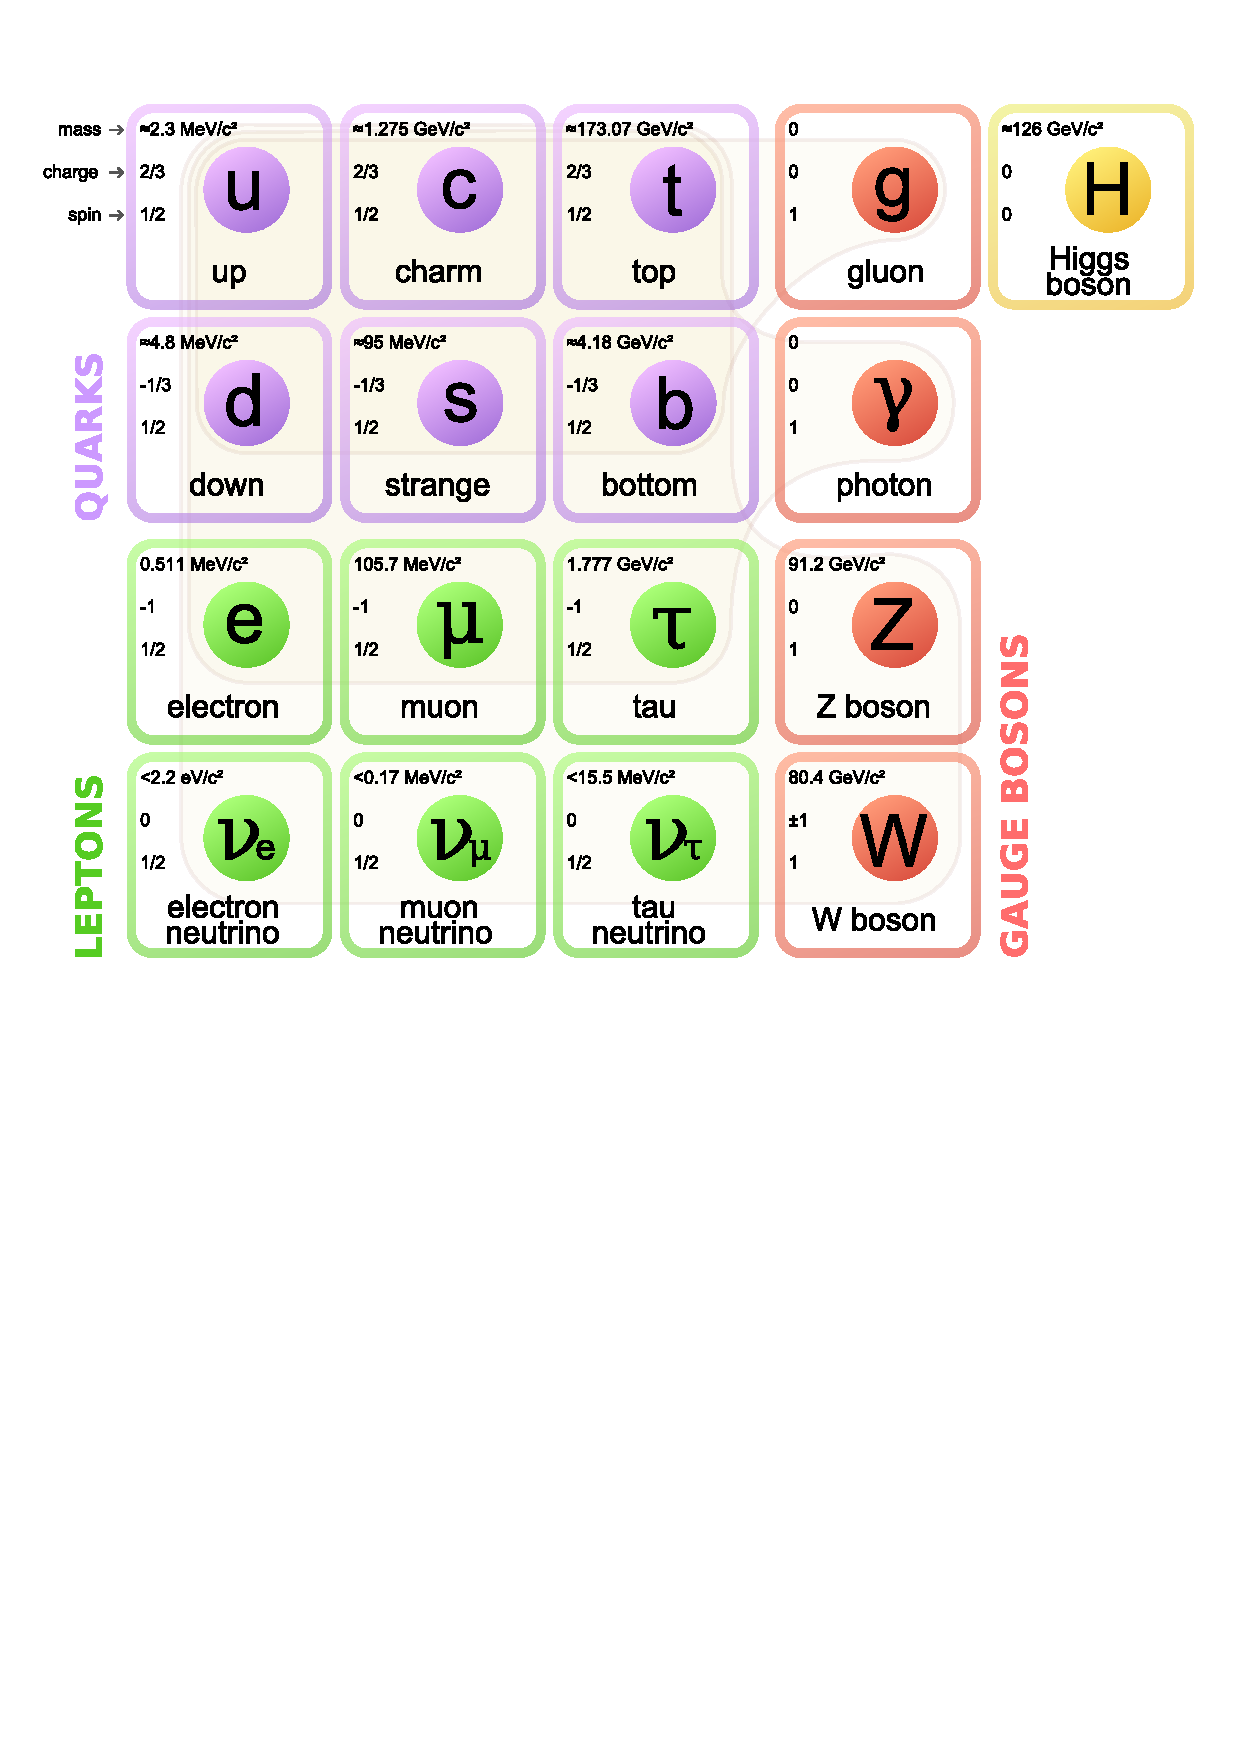
\includegraphics[width=12.cm]{./Version1/FigChapter1/SM}
\caption{Standard Model families of leptons and quarks as the gauge bosons}
\label{fig:sm}
\end{center}
\end{figure}

\textbf{Quantum Electro-Dynamics (QED)} describes how light and matter interact. This is the first theory where full agreement between quantum mechanics and special relativity is achieved. It was developed between 1946 and 1950 by Tomonaga Shinichiro, Julian S. Schwinger and Richard P. Feynmann. They were awarded the Nobel prize in 1965. \\

\textbf{Electroweak Theory (EW)} is the unified description of two of the four known fundamental interactions of nature: electromagnetism and the weak interaction. It first appeared in 1961, driven by Sheldon Lee Glashow, and was completed in 1967 by Abdus Salam and Steven Weinberg. They were awarded the Nobel prize in 1979. The first measurement of the existence of the weak bosons W$^{+}$, W$^{-}$ and Z$^{0}$ was performed in 1983, when they were produced and directly observed in Sp$\bar{p}$S collisions at CERN. During the next year the Nobel prize for this experimental result was assigned to Carlo Rubbia and Simon van der Meer. In 1999 Gerardus ?t Hooft and Martinus Veltman were awarded the Nobel prize for showing that the electroweak theory is renormalisable. \\

\textbf{Quantum Chromo-dynamics (QCD)} is the theory of the strong interaction (color force), describing the interactions between quarks and gluons which make up the hadrons. Starting from the classification of the large amount of particles discovered during the fifties, the original idea of the quark model by Gell-Mann (Nobel Prize in 1969) has been developed during the sixties until 1973, when David J. Gross, H. David Politzer and Frank Wilczek discovered the ?asymptotic freedom? property of the strong nuclear interaction (Nobel Prize in 2004).

\subsection{QCD and Quark-Gloun plasma}
The strong interaction is one of the four fundamental forces in nature, together with gravity, electromagnetism and the weak interaction. Its existence was postulated in the 1970s, to explain how the atomic nucleus was bound together despite the protons? mutual electromagnetic repulsion. This hypothesized force was called the strong force, which was believed to be a fundamental force that acted on the nucleons. It was later discovered that protons and neutrons were not fundamental particles, by means of deep inelastic experiments, but were made up of constituent particles (the quarks). The strong attraction between nucleons was the side-effect of a more fundamental force that bounds the quarks together in the protons and neutrons. Nowadays the strong inter- action is described through the formalism of a Quantum Field Theory. The particular theory describing this force is the Quantum Chromo-Dynamics (QCD), in analogy to the Quantum Electro-Dynamics (QED) that describes the electromagnetic interaction. In QED the electromagnetic force is mediated by photons, which carry no charge. Similarly, in QCD the gluons are the carriers of the strong force, but unlike the photon they carry color charge, meaning that they can interact with each other. In QED, the electrodynamic coupling constant is $\alpha$ = 1/137, whereas the QCD strong coupling constant, $\alpha_{s}$, can be 1 or larger. In quantum field theory when a coupling constant is much smaller than 1 the theory is said to be weakly coupled. When the coupling nears 1 the theory is strongly coupled, hence the name ?strong? force.
In QCD the strong interaction between two quarks can be described using the following potential:

\begin{equation}\label{label:potential}
V(r) = -4\frac{\alpha_{s}}{3r} + kr
\end{equation}

where r is the separation distance between the two quarks, $\alpha_{s}$ is the strong coupling constant, and $k$ is also a constant that is approximately 1 GeV/fm. The renormalization scale dependence of the effective QCD coupling $\alpha_{s}$ = $g^{2}_{s}$/4$\pi$ is controlled by the $\beta$-function:


 \begin{equation}\label{label:betaftn}
\mu \frac{\partial \alpha_{s}}{\partial \mu} = 2\beta(\alpha_{s}) = - \frac{\beta_{0}}{2\pi}\alpha_{s}^{2} - \frac{\beta_{1}}{4\pi^{2}}\alpha_{s}^{3} - \frac{\beta_{2}}{64\pi^{3}}\alpha_{s}^{4} - ...
\end{equation}
where
 \begin{equation}\label{label:b0}
\beta_{0} = 11 - \frac{2}{3}n_{f}
\end{equation}
 \begin{equation}\label{label:b1}
\beta_{1} = 51 - \frac{19}{3}n_{f}
\end{equation}
 \begin{equation}\label{label:b2}
\beta_{2} = 2857 - \frac{5033}{9}n_{f} + \frac{325}{27}n_{f}^{2}
\end{equation}

Here $n_{f}$ is the number of quarks with mass less than the energy scale $\mu$. In solving the differential equation \ref{label:betaftn} for $\alpha_{s}$,  a constant of integration is introduced. This constant is the fundamental constant of QCD that must de determined from experiment in addition to the quark masses. The most sensible choice for this constant is the value of $\alpha_{s}$ at a fixed-reference scale $\mu_{0}$. It has become standard to choose  $\mu_{0}$ = $M_{Z}$. At different
values of $\mu$, $\alpha_{s}$ can be obtained from 

 \begin{equation}\label{label:cal}
log(\frac{\mu^{2}}{\mu_{0}^{2}}) = \int_{\alpha_{s}(\mu_{0})}^{\alpha_{s}(\mu)} \frac{d\alpha}{\beta(\alpha)}
\end{equation}

It is also convenient to introduce the dimensional parameter $\Lambda $[MeV$^{-1}$], since it provides a parameterization of the $\mu$ dependence of $\alpha_{s}$. The definition of $\Lambda$ is arbitrary. One way to define it is to write the solution of Equation \ref{label:betaftn} as an expansion in inverse power of ln$(\mu^{2})$:
 
 \begin{equation}\label{label:expansions}
\alpha_{s} = \frac{4\pi}{\beta_{0}ln(\mu^{2}/\Lambda^{2})}[1 - \frac{2\beta_{1}}{\beta_{0}^{2}} \frac{ln[ln(\mu^{2}/\Lambda^{2})]}{ln(\mu^{2}/\Lambda^{2})} + \frac{4\beta_{1}^{2}}{\beta_{0}^{4}ln^{2}(\mu^{2}/\Lambda^{2})} \times ((ln[ln(\mu^{2}/\Lambda^{2})] - \frac{1}{2})^{2} + \frac{\beta_{2}\beta_{0}}{8\beta_{1}} - \frac{5}{4})]
\end{equation}


\begin{figure}[htbp]
\begin{center}
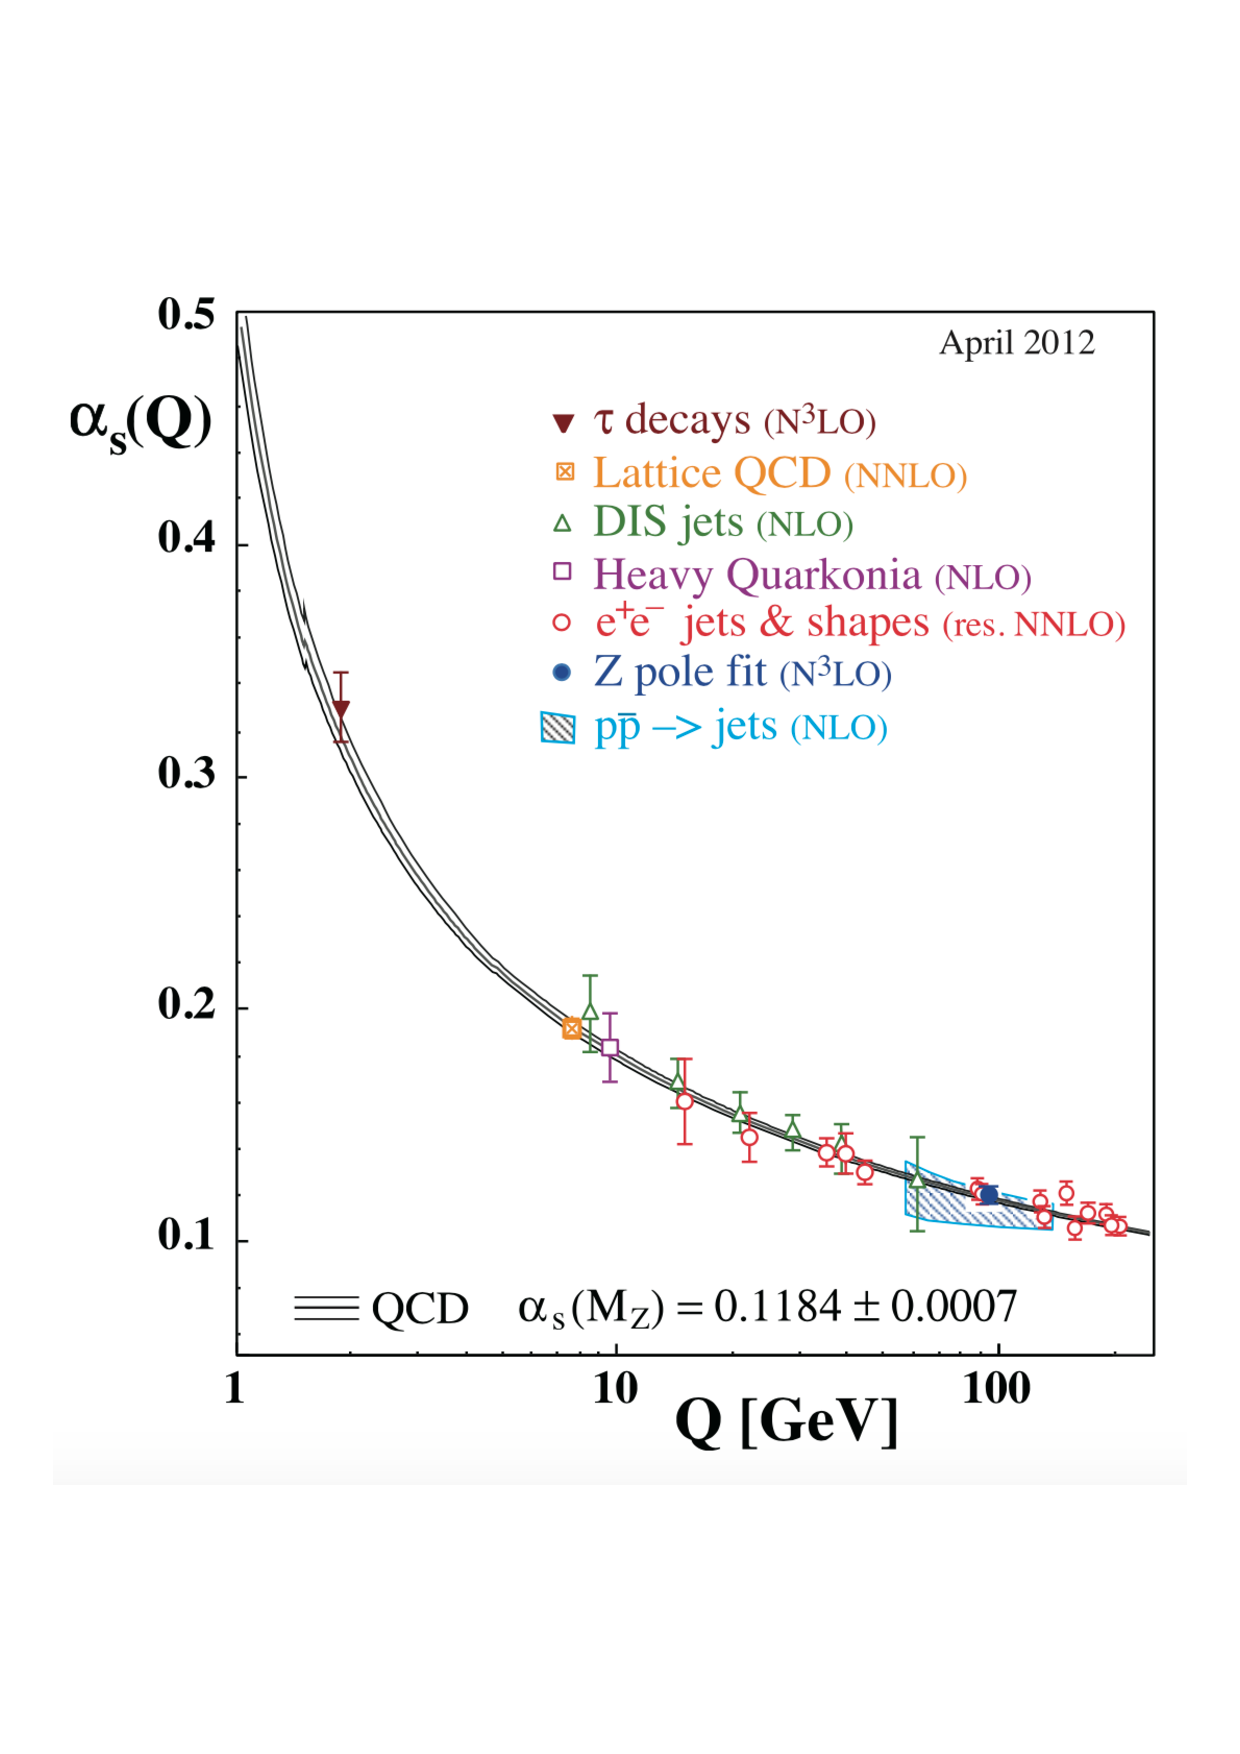
\includegraphics[width=12.cm]{./Version1/FigChapter1/QCD_alpha}
\caption{Summary of measurements of ?s as a function of the respective energy scale Q. The respective degree of QCD perturbation theory used in the extraction of ?s is indicated in brackets (NLO: next-to-leading order; NNLO: next-to-next-to leading order; res. NNLO: NNLO matched with resummed next-to-leading logs; N3LO: next-to-NNLO) \cite{cite:PDG}}
\label{fig:alpha}
\end{center}
\end{figure}

Experimentally, $\alpha_{s}$ has been measured at different scales ($\mu$). Figure \ref{fig:alpha} shows the measurement of $\alpha_{s}$ as a function of the respective energy scale $Q$ compared to the lattice QCD calculation.
Three very important properties of QCD arise from the running constant $\alpha_{s}$. They are confinement, asymptotic freedom, and (hidden) chiral symmetry. For large distance scales the second term in the potential equation (Equation \ref{label:expansions}) dominates. This means that the coupling between the two quarks is large, making it so that no free quarks are observed in nature, i.e. a quark never exists on its own for longer than 1/$\Lambda$QCD, where $\Lambda$QCD = 217 MeV. The up, down, strange, charm, and bottom quarks all hadronize on the time-scale 1/$\Lambda$QCD, the top quark decays before it has time to hadronize. Therefore, all but the top quark will be confined inside hadrons. Experimentally, no single quark in a color- triplet state has ever been observed.
Asymptotic freedom arises when the quarks are at a small distance from one another or with a large enough momentum transfer $Q$ ($\alpha_{s}$ $\rightarrow$ 0 as $\mu$ $\rightarrow$ $\infty$). The potential will go like 1/r and the effective coupling between the quarks decreases, allowing for a quasi-free quark. The third property is called chiral symmetry, also not observed in nature. It is a symmetry of QCD in the limit of vanishing quark masses. In this limit quarks are either left of right handed, such that the QCD Lagrangian is symmetric. However, when quarks are confined inside hadrons they have large dynamical masses, called constituent or QCD masses. Here the chiral symmetry is said to be ?broken? (or hidden). In the small ?s limit some quarks will have small mass, called current mass. In this limit, chiral symmetry is said to be (partially) restored.
In our world, quarks and gluons are confined inside hadrons. By significantly increasing the temperature and energy density the strong force holding the quarks and gluons together may be reduced, unbinding them from the hadrons. This phenomenon is known as "de-confinement". De-confinement implies that there exists a phase transition from a gas of hadrons to a new form of matter of free quarks and gluons, called the Quark-Gluon Plasma (QGP).

\newpage
\subsection{Heavy Ion Collisions}
In the case a QGP is formed, it will eventually expand because of its internal pressure. As the system expands it also cools. The space-time evolution of the expansion can be seen in Figure \ref{fig:freezeout} (right side). A and B represent the two incoming ion beams. After a pre- equilibrium phase a QGP is formed. As it expands, the system will eventually reach what is known as the critical temperature ($T_{c}$). At this point partons begin to hadronize and this will continue until the chemical freeze-out ($T_{ch}$) takes place, when inelastic collisions cease. At this stage the distribution of hadrons is frozen. As cooling and expansion continue the hadrons reach what is called thermal freeze out ($T_{fo}$). Here the elastic collisions stop and the hadrons carry fixed momenta. The QGP state can not be directly observed, because of its short lifetime. Instead, through experiment we measure the final state hadrons, which have a fixed momentum after $T_{fo}$. The observables of interest should tell us about the de-confinement and the thermodynamic properties of the matter. Moreover, experimental measurements include yields and \pt spectra of various particle species, azimuthal studies of high \pt particles, phase space distributions, and particle correlations.

\begin{figure}[htbp]
\begin{center}
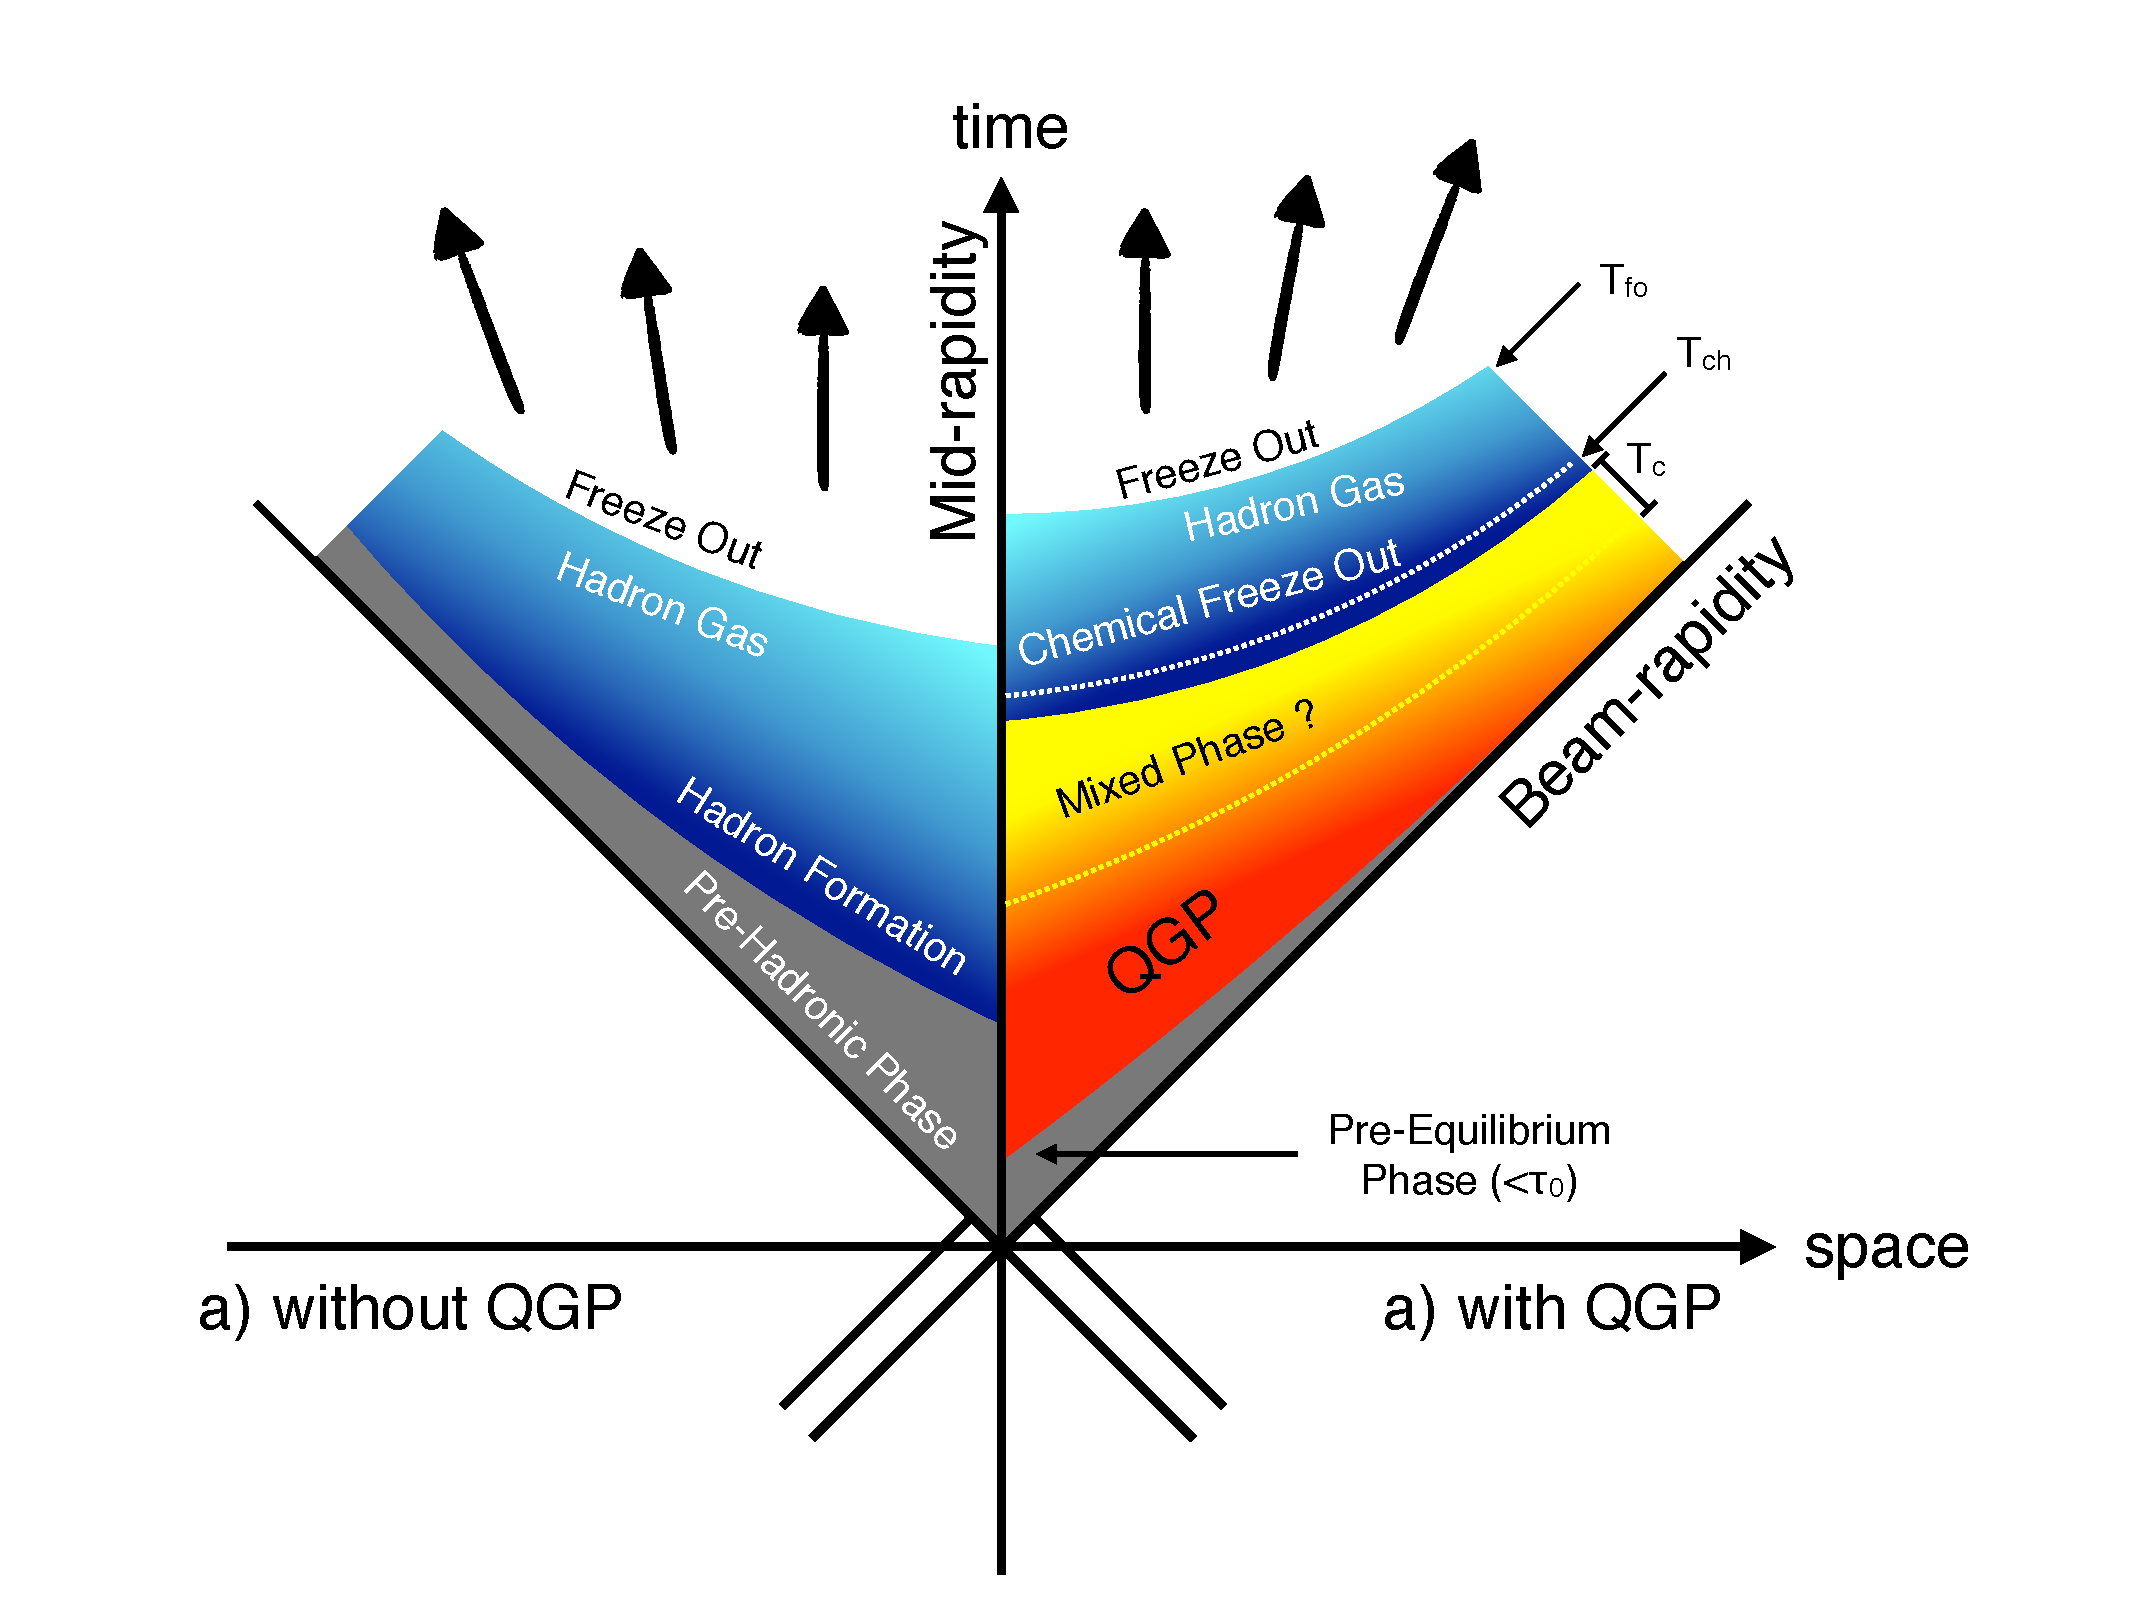
\includegraphics[width=10.cm]{./Version1/FigChapter1/FreezeOut}
\caption{Hydrodynamic evolution of a heavy ion collision with and without the formation of a QGP. }
\label{fig:freezeout}
\end{center}
\end{figure}

\newpage